%%% LaTeX Template: Article/Thesis/etc. with colored headings and special fonts
%%%
%%% Source: http://www.howtotex.com/

\documentclass[12pt]{article}


\usepackage{apuntes-estilo}
\usepackage{fancyhdr,lastpage}
\usepackage{color,colortbl}
\usepackage{verbatim}

\def\maketitle{

% Titulo 
 \makeatletter
 {\color{bl} \centering \huge \sc \textbf{
 El shell o intérprete de comandos \\ 
\large \vspace*{-8pt} \color{black} Guía básica de uso del shell
 \vspace*{8pt} }\par}
 \makeatother


% Autor
 \makeatletter
 {\centering \small 
 	Departamento de Ingeniería de Computadoras \\
 	Facultad de Informática - Universidad Nacional del Comahue \\
 	\vspace{20pt} }
 \makeatother

}

% Custom headers and footers
\fancyhf{} % clear all header and footer fields
\fancypagestyle{plain}{\fancyhf{}}
  	\pagestyle{fancy}
 	\lhead{\footnotesize El Intérprete de comandos (shell) - Departamento de Ingeniería de Computadoras}
 	\rhead{\footnotesize \thepage\ }	% ''Page 1 of 2''

\def\ti#1#2{\texttt{#1} & #2 \\ }



\begin{document}

\thispagestyle{empty}
\maketitle
\setlength{\parindent}{0pt}

\section{Intérprete de comandos: Shell}

El intérprete de comandos es el programa que recibe lo que se escribe en la terminal y lo convierte en instrucciones para el sistema operativo.

En otras palabras el objetivo de cualquier intérprete de comandos es ejecutar los programas que el usuario escribe en el \texttt{prompt} del mismo. 
El \texttt{prompt} es una indicación que muestra el intérprete para anunciar que espera una orden del usuario. Cuando el usuario escribe una orden, 
el intérprete ejecuta dicha orden. En dicha orden, puede haber programas internos o externos: Los programas internos son aquellos que vienen 
incorporados en el propio intérprete, mientras que los externos son programas separados (ej: aplicaciones de /bin/ls,/usr/bin/top,...).\cite{curlin}

En el mundo Linux/Unix existen tres grandes familias de Shells como se muestra en la tabla a continuación. Estas se diferencian entre 
sí básicamente en la sintaxis de sus comandos y en la interacción con el usuario.

\definecolor{tcA}{rgb}{1,0.972549,0.717647}
\begin{center}
\begin{tabular}{|l|l|l|}\hline
\rowcolor{tcA}
\textbf{Tipo de shell} & \textbf{Shell estándar} & \textbf{Implementación libre}\\\hline
AT\&T Bourne shell & sh & ash, bash, bash2\\\hline
Berkeley ``C'' shell & csh & tcsh\\\hline
AT\&T Korn shell & ksh & pdksh, zsh\\\hline
Otros interpretes  & -- & esh, gush, nwsh\\\hline
\end{tabular}
\end{center}

\subsection{Sintaxis de los comandos}

Los comandos tienen la siguiente sintaxis:

\texttt{\# programa arg1 arg2 ... argn}

Se observa que, en la ``línea de comandos'', se introduce el programa seguido de uno o varios argumentos. 
Estos argumentos representarán opciones o argumentos de entrada para el programa invocado por el shell. 

\fcolorbox{black}{grey}{
\parbox[t]{1.0\linewidth}{ \vspace*{0.4cm}
{\bf Ejemplo 1:} \\
En este caso el programa \texttt{cat} recibe un argumento \texttt{archivo.txt}
sobre el cuál realizar la acción del programa.  \\
\texttt{
\$ cat archivo.txt \\
archivo de texto de prueba\\
otra linea de prueba\\
}
\vspace*{0.4cm} } }

\fcolorbox{black}{grey}{
\parbox[t]{1.0\linewidth}{ \vspace*{0.4cm}
{\bf Ejemplo 2:} \\
A continuación el primer argumento constituye una opción que modifica la forma normal 
de operar del comando \texttt{cat}, el segundo argumento es el archivo de entrada sobre
el cual realizar la acción. La opción \texttt{-n} le indica a \texttt{cat} que debe 
imprimir el número de línea además del contenido del archivo. (\texttt{man cat}) \\
\texttt{
\$ cat -n archivo.txt \\
     1	archivo de texto de prueba\\
     2	otra linea de prueba\\
}
\vspace*{0.4cm} } }

En ocasiones, cuando la línea del comando se torna demasiado extensa, es conveniente dividirla
en dos o mas líneas. Para ello e separa cada línea con el carácter barra invertida (\textbackslash), 
el cuál le indica al intérprete que no hemos finalizado nuestro comando y que lo continuaremos 
en la próxima línea. Así al presionar ``\texttt{ENTER}'' luego de una barra invertida, el comando 
no será ejecutado inmediatamente, sino que el intérprete quedará esperando el resto de la invocación. 

También es posible ejecutar más de un comando en la misma línea separándolos con punto y coma (;). 

\fcolorbox{black}{grey}{
\parbox[t]{1.0\linewidth}{ \vspace*{0.4cm}
{\bf Ejemplo:}\\ 
\texttt{\# date ; echo esto es una prueba \textbackslash \\
con barra invertida \\
mié mar 20 20:30:57 ART 2013 \\
esto es una prueba con barra invertida \\
\#}
\vspace*{0.4cm} } }

\subsection{Variables de entorno}

Una variable de entorno es un nombre asociado a una cadena de caracteres. Dependiendo de la variable, su utilidad puede ser distinta. 
Algunas son útiles para no tener que escribir muchas opciones al ejecutar un programa, otras las utiliza el propio shell (PATH, PS1,...). 

La tabla muestra la lista de variables más comunes:

\begin{center}
\begin{tabular}{|l|l|}\hline
\rowcolor{tcA}
Variable & Descripción \\\hline
DISPLAY & Donde aparecen la salida de X-Windows (sistema gráfico)\\\hline
HOME & Nombre del directorio personal del usuario\\\hline
HOSTNAME & Nombre de la máquina\\\hline
PATH & Lista de directorios de búsqueda de programas\\\hline
PS1 & Formato del \texttt{prompt}\\\hline
SHELL & Intérprete de comandos predeterminado\\\hline
TERM & Tipo de terminal\\\hline
EDITOR & Editor invocado de manera predeterminada\\\hline
USER & Nombre del usuario\\\hline
PAGER & Paginador utilizado de manera predeterminada\\\hline
\end{tabular}
\end{center}

El nombre y la forma de definir una variable de entorno cambia con el interprete de comandos.
Por ejemplo en el shell \texttt{bash} se definen ejecutando el siguiente comando: \texttt{export \textless NOMBRE\_DE\_VARIABLE\textgreater=\textless valor\_de\_la\_variable\textgreater}.

Para conocer el valor de las variables de entorno ejecute el comando \texttt{env} o bien imprima su valor
a través del comando \texttt{echo \$\textless NOMBRE\_DE\_VARIABLE\textgreater}


\fcolorbox{black}{grey}{
\parbox[t]{1.0\linewidth}{ \vspace*{0.4cm}
{\bf Ejemplo:}
Si la variable de entorno \texttt{LANG} se encuentra definida con el valor \texttt{es\_AR.UTF-8}, algunos programas, como por ejemplo \texttt{man}, interpretarán que el lenguaje en que el usuario actual está trabajando es español, y modificará su comportamiento de acuerdo a ello. En el caso del programa \texttt{man}, de estar disponibles, mostrará las páginas del manual requeridas en idioma español. Mientras que, si definimos la variable de entorno \texttt{LANG=en\_US.UTF-8}, man mostrará las páginas del manual en inglés.
\vspace*{0.4cm} } }

\subsection{Comodines}
Los comodines son caracteres que cuentan con un significado especial para el shell (subconjunto de un conjunto 
amplio de metacaracteres con significado especial). 
Explicaremos brevemente el uso de algunos comodines (wildcards en inglés). 
Al igual que en los juegos de cartas, los comodines en el shell indican opción, o patrón de coincidencia. 
Aprendamos acerca de su uso a través de una serie de ejemplos: 

\textbf{El comodín ``*''}:
Concuerda con cualquier cadena de cero o mas caracteres en archivos. 
\begin{itemize}
\item \texttt{ls *} indica al comando \texttt{ls} aplicar su función a \textit{todos} los archivos y 
directorios en el directorio actual, excluyendo los archivos y directorios ocultos. Nótese la diferencia
con \texttt{ls} sin argumentos, que solo listara el contenido del directorio actual. 
\item El comando \texttt{ls *.pdf} aplicará la función a \textit{todos} los archivos que finalicen en ``.pdf''. 
\item El comando \texttt{cat capítulo*.txt} aplicará su función, a todos los archivos tales que comiencen con 
``capítulo'' y finalicen con ``.txt''. Por ejemplo: capítulo01.txt, capítulo123.txt, capítuloHola.txt, etc. coincidirán con el 
patrón, mientras que capítulo02, hola.txt no lo harán.  
\end{itemize} 

\textbf{El comodín ``?''}:
Concuerda con cualquier caracter individual en archivos. 
\begin{itemize}
\item El comando \texttt{ls capítulo?.txt} aplicará su función de listado a archivos que posean un caracter
cualquiera entre ``capítulo'' y ``.txt''. Así por ejemplo capítulo1.txt coincide con este patrón mientras que 
capítulo123.txt no lo hará. 
\end{itemize} 

\textbf{El comodín ``[ccc]''}:
Concuerda con cualquier caracter individual de ``ccc'' en archivos; son legales los intervalos como 
0-9 o a-z. 
\begin{itemize}
\item \texttt{ls capítulo[0-9].txt} aplicará su función de listado a cualquier archivo que coincida 
con ese patrón. Por ejemplo capítulo9.txt coincidirá, mientras que capítuloa.txt no lo hará. 
\end{itemize} 

\fcolorbox{black}{grey}{
\parbox[t]{1.0\linewidth}{ \vspace*{0.4cm}
{\bf Observación 1:}
El shell expande los comodines \textbf{antes} de ejecutar el comando en cuestión, por 
lo que el comando recibirá la lista de argumentos ya expandidos.
\vspace*{0.4cm} } }

\fcolorbox{black}{grey}{
\parbox[t]{1.0\linewidth}{ \vspace*{0.4cm}
{\bf Observación 2:}
¿Qué sucede si uno de estos comodines forma parte del nombre de archivo? Por ejemplo si nuestro 
archivo se llama ``capítulo[1-2].txt''. En este caso es necesario ``escapar'' el metacaracter 
anteponiendo una contra barra ``\textbackslash'' al mismo. Por ejemplo: \texttt{cat 
capítulo\textbackslash[1-2\textbackslash].txt} mostraría el contenido del archivo, de otro modo 
intentaría mostrar el contenido de archivos con nombre capítulo1.txt y captítulo2.txt.
\vspace*{0.4cm} } }


\section{Redirección}

Una vez hemos aprendido a utilizar algunos de los comandos del sistema, es muy probable que en 
algunos casos nos interese utilizarlos de manera simultánea para agilizar las 
acciones que queremos realizar. Una operación muy interesante consiste en poder 
tomar la salida de un comando para que sirva de entrada a otro y procesarla adecuadamente. 
El sistema operativo utiliza un mecanismo de pipes (tuberías), que nos permite redirigir las salidas 
de cualquier comando o programa hacia donde queramos. Su funcionamiento es muy simple: se trata de poner el 
carácter ``\textbar'' entre los comandos, de manera que la salida del primero sirve como
 entrada para el segundo.

Ejemplo: al escribir el comando 
\texttt{echo campo1:campo2:campo3:campo4}, lo único que conseguiríamos sería que por 
pantalla nos apareciera ``\texttt{campo1:campo2:campo3:campo4}''. Si de esta salida sólo 
quisiéramos tomar el  ``\texttt{campo3}'', podríamos redirigirla con un pipe hacia el 
comando cut, para que seleccione únicamente el campo que nos interesa de la siguiente manera: 
\texttt{echo campo1:campo2:campo3:campo4 | cut -d: -f 3}. 

En la siguiente figura podemos ver este ejemplo de manera gráfica:

\begin{center}
 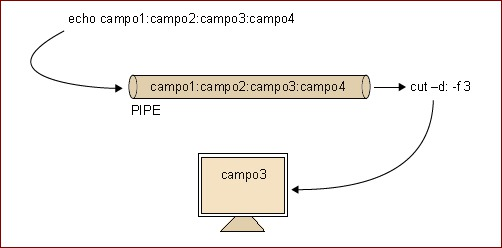
\includegraphics{./img/redireccionamiento.jpg}
 % redireccionamiento.gif: 502x248 pixel, 72dpi, 17.71x8.75 cm, bb=0 0 502 248
\end{center}


Naturalmente, podemos conectar tantas tuberías como necesitemos para realizar 
acciones más prácticas que la que acabamos de ver. Otro tipo de 
redireccionamientos muy prácticos son aquellos que están relacionados con los 
ficheros. Este tipo de redireccionamiento nos permite tomar toda la salida de 
un comando o programa y guardarla en un fichero utilizando el carácter ``\textgreater'', 
igual que hacíamos con ``\textbar''. Por ejemplo, si queremos guardar en un nuevo 
fichero todo lo que vayamos escribiendo hasta apretar ``Ctrl + C'', podríamos 
utilizar lo siguiente: \texttt{cat > prueba.txt}. Con ``\textgreater \textgreater'' 
podemos hacer exactamente 
lo mismo, pero en lugar de crear siempre el nuevo fichero, si este ya 
existiera, se añadiría la información al final del mismo. Con ``\textless'' el 
redireccionamiento se realiza en sentido contrario, de modo que el 
contenido del fichero que le indicamos se dirigirá hacia el comando o programa 
señalado.

Un aspecto muy interesante que debemos conocer es que en sistemas tipo UNIX 
se separa la salida normal de un programa con la de los errores. Aunque de  
manera predeterminada las dos salidas están dirigidas a la consola donde 
se ha ejecutado el programa, podemos manipularlas para que se dirijan hacia 
donde queramos. Para ver esto de manera práctica, intentamos borrar un fichero 
que no existe con la siguiente instrucción: \texttt{rm fichero \textgreater resultados}. Aunque 
estamos redireccionando la salida del comando hacia el fichero de resultados, 
por pantalla nos aparecerá un mensaje de error indicando que no se ha encontrado 
el fichero. Esto se debe a que de manera predeterminada los redireccionamientos sólo aceptan 
la salida estándar del programa y no la de error, que de manera predeterminada también se 
muestra por pantalla. Para redirigir la salida de error, deberíamos indicar, 
antes del carácter ``\textgreater'' el número ``2'', que es la salida de error (la ``1'' es la 
normal). De esta manera, ejecutando rm fichero 2 \textgreater resultados sí que conseguiríamos
que la salida se redirigiera al archivo de resultados. También podemos guardar 
la salida normal y la de errores en dos ficheros diferentes: rm fichero 1\textgreater resultados 2\textgreater 
errores. Si por el contrario quisiéramos que todas las salidas se dirigieran
 hacia un mismo archivo, podríamos utilizar ``\textgreater\&''. Además, con el carácter ``\&'' 
podemos encaminar salidas de un tipo hacia otras; por ejemplo, si quisiéramos 
encaminar la salida de errores hacia la normal, podríamos indicarlo del 
siguiente modo: 2\textgreater\&1.

Es importante tener en cuenta que el orden de los redireccionamiento es 
significativo: siempre se ejecutan de izquierda a derecha.

\section{Filtros: grep}
Existen una familia de comandos cuya función es aplicar filtros a la entrada que 
reciben: grep, egrep, sed, fgrep, son algunos de ellos. En este apunte desarrollaremos brevemente el 
comando \texttt{grep} y \texttt{egrep} que son de gran utilidad. Ambos muestran 
líneas que concuerdan con un patrón. 

Los siguientes ejemplos utilizan el archivo \texttt{lista.txt} como argumento, cuyo 
contenido es: 

\texttt{Arup:India:medico clinico \\
Francisco:Italia:enfermero \\
Jean:Francia:medico cardiologo \\
Rajesh:India:Administrador de sistemas \\
Patricio:Argentina:abogado\\
Isabel:Argentina:abogada\\
Mia:Francia:enfermera\\
Jack:Estados Unidos:abogado\\
Joseph:estados unidos:administrativo\\
Andrea:argentina:medica ginecologa
}

Ejemplos con \texttt{grep}:
\texttt{
\begin{itemize}
\item  \$ grep medico lista.txt \\
Arup:India:medico clinico \\
Jean:Francia:medico cardiologo \\ 
\item \$ grep medica lista.txt \\
Andrea:argentina:medica ginecologa \\
\item \$ grep medic lista.txt \\
Arup:India:medico clinico \\
Jean:Francia:medico cardiologo \\
Andrea:argentina:medica ginecologa 
\item \$ grep argentina lista.txt \\
Andrea:argentina:medica ginecologa 
\item \$ grep \textbf{-i} argentina lista.txt  \\
Patricio:Argentina:abogado \\
Isabel:Argentina:abogada \\
Andrea:argentina:medica ginecologa
\item \$ grep \textbf{-c} argentina lista.txt \\
1 
\item \$ grep \textbf{-ci} argentina lista.txt \\
3
\item \$ grep -vi argentina lista.txt \\
Arup:India:medico clinico \\
Francisco:Italia:enfermero \\
Jean:Francia:medico cardiologo\\ 
Rajesh:India:Administrador de sistemas \\
Mia:Francia:enfermera\\
Jack:Estados Unidos:abogado\\
Joseph:estados unidos:administrativo
\end{itemize}
}

Ejemplos con \texttt{egrep}:
\texttt{
\begin{itemize}
\item  \$ egrep 'argentina|India' lista.txt \\
Arup:India:medico clinico \\
Rajesh:India:Administrador de sistemas \\
Andrea:argentina:medica ginecologa
\item \$ egrep -i 'argentina|India' lista.txt \\
Arup:India:medico clinico \\
Rajesh:India:Administrador de sistemas \\
Patricio:Argentina:abogado \\
Isabel:Argentina:abogada \\
Andrea:argentina:medica ginecologa
\item \$ egrep -ci 'argentina|India' lista.txt \\
5
\end{itemize}
}

\subsection*{Filtros y redirección}
Ahora que conocemos el uso básico de filtros y redirección, utilicemos ambos 
conocimientos en conjunto. Alimentemos los filtros con salidas de otros comandos
utilizando la redirección. Veamos algunos ejemplos: 

\textit{Identificando al proceso init del sistema:  }

\begin{verbatim}
$ ps -ef |grep init 
root     1     0  0 19:21 ?        00:00:01 init [2]  
pepe  6202     1  0 19:31 ?        00:00:00 kdeinit4: kdeinit4 Running...
pepe  6203  6202  0 19:31 ?        00:00:00 kdeinit4: klauncher [kdeinit] --fd=8
pepe  6205     1  0 19:31 ?        00:00:00 kdeinit4: kded4 [kdeinit]  
pepe  9904  9748  0 22:46 pts/2    00:00:00 grep init
\end{verbatim}

\textit{¿Cuántos intérpretes \texttt{bash} se encuentran en ejecución?:}
\begin{verbatim}
$ ps -ef |grep -v grep| grep -c bash 
7
\end{verbatim}
Pregunta: ¿por qué aparece \texttt{grep -v grep} en el comando anterior?

\textit{¿Ha iniciado sesión el usuario pepe?:}
\begin{verbatim}
$ who |grep pepe
\end{verbatim}

\textit{Mostrar los procesos de los usuarios maria y antonio:}
\begin{verbatim}
$ ps -ef | egrep '^maria |^antonio '
\end{verbatim}

Nota: en la expresión anterior los metacaracteres `` \^ '' y `` \textbar '' son 
interpretados por el comando grep y no por el shell. Esto se debe a que 
todo lo encerrado entre `` ' '' (comillas simples) es interpretado 
literalmente por el shell.



\section{Moviéndonos por la estructura de directorios}

Para movernos por la estructura de directorios debemos utilizar los comandos para 
listar contenidos y cambiar de carpeta. Cuando entramos en el sistema, es usual 
que el programa \texttt{login} nos sitúe en nuestro directorio home, que generalmente se suele 
referenciar con el carácter ``\textasciitilde''. Si queremos ver lo que hay en el 
directorio donde estamos situados, podemos listar los contenidos utilizando el 
comando \texttt{ls}. Debemos tener en cuenta que por defecto el comando no nos muestra los 
archivos que empiezan por un punto (archivos ocultos). Con la opción \texttt{-a} nos mostraría 
absolutamente todos los archivos y directorios, incluidos los ocultos. En todos los directorios existe una entrada 
``.'' y otra ``..''. El punto es la referencia al directorio actual, mientras 
que los dos puntos seguidos hacen referencia al directorio inmediatamente superior 
(en el árbol de jerarquías) al actual. Naturalmente, cuando estamos situados en 
la raíz del sistema de ficheros, la entrada ``..'' no existirá porque nos encontramos 
en el nivel superior.

Para cambiar de directorio podemos utilizar el comando \texttt{cd}. Si no le pasamos ningún argumento, 
de manera predeterminada nos situará en nuestro directorio home. Generalmente, se le suele indicar 
dónde queremos ir, pasándolo de forma absoluta o relativa. De forma relativa significa que partiremos 
especificando el directorio desde el directorio donde estamos situados en el momento de ejecutar el comando. 
Mientras que, de forma absoluta siempre partimos de la raíz.

\fcolorbox{black}{grey}{
\parbox[t]{1.0\linewidth}{ \vspace*{0.4cm}
{\bf Ejemplo}. Si estamos en el
directorio \texttt{/usr/bin/} y queremos ir al \texttt{/root/}, para indicarlo de manera relativa deberíamos 
introducir el siguiente comando: \texttt{cd ../../root} (los dos primeros puntos indican \texttt{/usr/} y los siguientes, 
la raíz / del sistema, a partir de la cual ya podemos acceder a \texttt{/root/}). 
Para hacer lo mismo de manera absoluta utilizaríamos el comando: \texttt{cd /root}. 
\vspace*{0.4cm} } }

Para saber en qué directorio estamos, podemos utilizar el comando \texttt{pwd}.

\section{Obteniendo ayuda en linea}
Como se explicó en la sección sobre sintaxis, los comandos suelen aceptar opciones y argumentos, 
que permiten modificar su comportamiento predeterminado e indicar entradas sobre las que 
realizar la tarea. Sin embargo sería imposible para un administrador recordar todas las opciones, 
o incluso la forma de sus argumentos. 

Del mismo modo, esta información es necesaria para los archivos de configuración del sistema, sería
difícil recordar cuál es el orden de los campos de la base de datos de usuarios locales(\texttt{/etc/passwd}),
etc. Por ello, el propio sistema incorpora un mecanismo de manuales, accesibles en linea de comandos, 
con el que podemos consultar casi todos estos aspectos de los programas, utilidades, comandos y 
configuraciones existentes. 

El comando a través del cual accedemos a estos manuales es \texttt{man}, que nos muestra en la terminal 
el manual del programa que se le indica como argumento. Esta 
documentación se pagina (o muestra en secuencia de páginas) por medio del programa \texttt{less} o 
\texttt{more} (comportamiento que puede modificarse a través de la variable de entorno PAGER), con el 
que podemos desplazarnos hacia delante y hacia atrás con las teclas de ``AvPág'' y ``RePág'', buscar 
una palabra con el carácter ``/'' seguido de la palabra (``n'' nos sirve para buscar las siguientes 
ocurrencias y ``N'' para las anteriores), ``q'' para salir, etc. 

Los manuales del sistema están divididos en diferentes secciones según su naturaleza:
\begin{enumerate}
\item   Programas ejecutables y scripts del intérprete de órdenes
\item   Llamadas del sistema (funciones servidas por el núcleo)
\item   Llamadas de la biblioteca (funciones contenidas en las  bibliotecas
           del sistema)
\item   Ficheros especiales (se encuentran generalmente en /dev)
\item   Formato de ficheros y convenios p.ej. /etc/passwd
\item   Juegos
\item   Paquetes de macros y convenios p.ej. man(7), groff(7).
\item   Órdenes  de  administración  del  sistema (generalmente solo son para
           root)
\item   Rutinas del núcleo (no es estándar).
\end{enumerate}
	 

Si hay más de un manual disponible para una misma palabra, podemos especificar
a cuál nos referimos utilizando el número correspondiente de la sección deseada 
antes de la palabra. Como los otros comandos, man tiene opciones documentadas 
en su propio manual (\texttt{man man}), a partir de las cuales podemos realizar 
búsquedas automáticas, crear un fichero del manual en formato imprimible, etc. 
Una de estas opciones, de gran utilidad, nos permite identificar manuales que 
mencionan una palabra, la opción \texttt{-k}. Así, si no recordamos con exactitud
el nombre de un comando, podemos invocar \texttt{man -k} y una palabra clave que 
sabemos a la cual el manual 
hará referencia (el comando \texttt{apropos} realiza una tarea similar). 

\fcolorbox{black}{grey}{
\parbox[t]{1.0\linewidth}{ \vspace*{0.4cm}
{\bf Ejemplo:}
\texttt{man passwd} muestra la información del comando passwd que permite cambiar 
la contraseña de un usuario del sistema, mientras que, \texttt{man 5 passwd} muestra
el manual acerca del formato del archivo \texttt{/etc/passwd} que contiene la base 
de datos de usuarios locales. 
\vspace*{0.4cm} } }
	

Si el manual no nos proporciona toda la información que necesitamos, podemos 
usar el comando \texttt{info}, que provee información adicional al manual. Por otra parte
si sólo queremos tener una breve referencia de lo que hace un determinado programa, 
biblioteca, etc., podemos utilizar el comando \texttt{whatis} ó la opción \texttt{--help o -h}
soportada por la gran mayoría de los comandos.


\section{Licencia}

Este material es una obra derivada de los siguientes textos:

``Sistema operativo GNU/Linux Básico'' \footnote{http://materials.cv.uoc.edu/continguts/XW07\_M2102\_02309/index.html}

© Autores: Joaquín López Sánchez-Montañés, Sofia Belles Ramos, Roger Baig i Viñas i Francesc Aulí Llinàs

© 2008, FUOC. Se garantiza permiso para copiar, distribuir y modificar este documento según los
términos de la GNU Free Documentation License, Version 1.2 o cualquiera posterior publicada por la
Free Software Foundation, sin secciones invariantes ni textos de cubierta delantera o trasera. Se dispone
de una copia de la licencia en el apartado ``GNU Free Documentation License'' de este documento.

\begin{thebibliography}{1}
\bibitem[CurLinux]{curlin} ``Curso de Linux''.1999 Gómez, Ahijado, Flores.\\ 
http://www.ibiblio.org/pub/Linux/docs/LuCaS/Tutoriales/CURSOLINUX/\\curso\_linux/curso\_linux.html
\end{thebibliography}

\end{document}
